\section{Аналитический раздел}

\subsection{Формализация задачи}

Цель данной работы -- написать драйвер геймпада Logitech F310 для использования его в качестве мыши и клавиатуры.

Для достижения поставленной цели необходимо:

\begin{itemize}[leftmargin=1.6\parindent]
    \item[---] рассмотреть устройство подсистемы USB,
    \item[---] проанализировать протокол взаимодействия геймпада,
    \item[---] разработать загружаемый модуль ядра,    
    \item[---] провести исследование разработанного драйвера.
\end{itemize}

\subsection{Драйверы устройств в ОС Linux}

Прикладные программы не могут обращаться к устройствам напрямую. Вся работа с устройствами должна происходить с использованием средств, предоставляемых операционной системой. Реализация взаимодействия операционной системы с новым внешним устройством требует написания драйвера -- управляющей программы.

Драйверы устройств играют особую роль в ядре Linux.
Они полностью скрывают детали того, как работают устройства, предоставляя интерфейс для взаимодействия с ними. Ролью драйвера устройства является сопоставление набора стандартизированных вызовов с операциями, специфичными для конкретного устройства.

Драйверы могут быть созданы отдельно от остальной части ядра и подключены во время выполнения, когда это необходимо.

\subsection{Подсистема USB}

Универсальная последовательная шина (USB) -- это соединение между компьютером и рядом периферийных устройств. Первоначально протокол USB был создан для замены широкого спектра медленных шин -- параллельных, последовательных и клавиатурных подключений -- одним типом шины, к которому могли бы подключаться все устройства.

В ядре операционной системы Linux имеется подсистема предназначенная для работы с USB-устройствами \cite{usb-basics}. Так как целевое устройство -- геймпад -- имеет USB интерфейс, в дальнейшем будет использована именно эта подсистема.

\clearpage

\begin{figure}[ht]
    \centering
    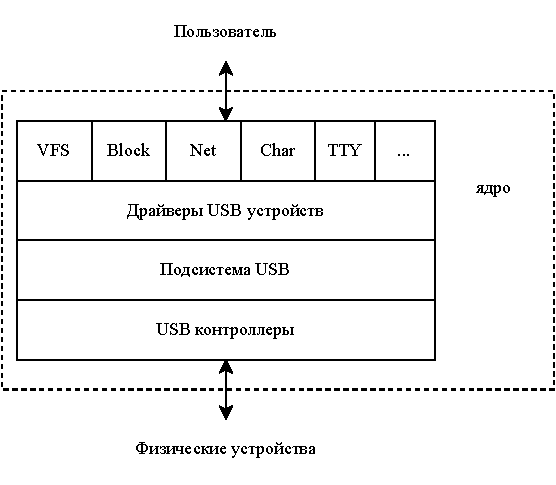
\includegraphics[width=0.8\linewidth]{img/usb-overview.pdf}
    \caption{Общее представление подсистемы USB}
\end{figure}

Для регистрации нового драйвера необходимо проинициализировать структуру \texttt{usb\_driver} и вызвать функцию \texttt{usb\_register}. По окончании работы с устройством, драйвер можно снять с учета посредством вызова функции \texttt{usb\_deregister}. 

\begin{small}
\begin{verbatim}
struct usb_driver {
    const char *name;
    int (*probe)(struct usb_interface *intf, struct usb_device_id *id);
    void (*disconnect) (struct usb_interface *intf);
    const struct usb_device_id *id_table;
    /* ... */
};

int usb_register(struct usb_driver *driver);
void usb_deregister(struct usb_driver *driver);
\end{verbatim}
\end{small}

Таблица \texttt{id\_table} предоставляет подсистеме информацию о том, какие именно устройства могут управляться регистрируемым драйвером.

Функции \texttt{probe} и \texttt{disconnect} вызываются соответственно в моменты подключения и отключения устройства, соответствующего данному драйверу.

\subsection{Подсистема ввода}

Подсистема ввода -- это уровень абстракции между устройствами ввода (клавиатура, мышь, геймпад и т. д.) и обработчиками ввода. Устройства ввода фиксируют входные данные от действий пользователя и генерируют входные события. Входные события проходят через подсистему ввода и отправляются заинтересованным обработчикам. Ядро ввода обеспечивает сопоставление "многие ко многим"\, между устройствами ввода и обработчиками событий.

Список наиболее распространенных типов событий, генерируемых с использованием подсистемы ввода:

\begin{itemize}[leftmargin=1.6\parindent]
    \item[---] \texttt{EV\_KEY} -- используется для описания изменений состояния клавиатур, кнопок или других устройств, похожих на клавиши;
    \item[---] \texttt{EV\_REL} -- используется для описания изменения значения относительной оси, например, перемещения мыши на 5 единиц влево;
    \item[---] \texttt{EV\_ABS} -- используется для описания изменений значений абсолютной оси, например, описания координат касания на сенсорном экране.
\end{itemize}

Для реализации управления мышью через геймпад можно использовать джойстики (один для перемещения мыши, второй для управления колесиком). Кнопки геймпада A и B можно назначить на кнопки мыши (левую и правую соответственно).

Для использования возможностей подсистемы ввода необходимо зарегистрировать драйвер устройства ввода. Создание структуры драйвера может быть выполнено вызовом одной из функции

\begin{small}
\begin{verbatim}
struct input_dev *input_allocate_device(void);
struct input_dev *devm_input_allocate_device(struct device *dev);
\end{verbatim}
\end{small}

Вторая функция использует механизм управляемых ресурсов устройств. Это позволяет сократить количество ошибок, связанных с очищением памяти после использования, в связи с применением счетчика ссылок. Для описания ресурсов устройства в ядре имеется специальная структура \texttt{devres}.

\begin{small}
\begin{verbatim}
typedef void (*dr_release_t)(struct device *dev, void *res);

struct devres_node {
    struct list_head entry;
    dr_release_t release;
    const char *name;
    size_t size;
};

struct devres {
    struct devres_node node;
    u8 __aligned(ARCH_KMALLOC_MINALIGN) data[];
};
\end{verbatim}
\end{small}

При удалении структуры устройства из системы, все связанные ресурсы будут освобождены посредством вызова функций \texttt{dr\_release\_t}.

\subsubsection{Перемещение курсора}

Изменение положения курсора на экране происходит посредством генерирования события типа \texttt{EV\_REL}. Согласно спецификации геймпада, движение джойстиков генерирует события типа \texttt{EV\_ABS}. В связи с этим, реализация движения курсора будет некорректной при простой замене одного типа события на другой -- фиксация джойстика в смещенном положении не будет приводить к поступлению новых URB блоков и генерированию новых событий перемещения мыши, и как следствие не будет происходить изменение положения курсора.

Для решения изложенной проблемы необходимо использовать таймер, который должен с постоянной периодичностью генерировать события при возникновении описанной ситуации. Для работы с таймером в ядре существует структура \texttt{timer\_list}.

\begin{small}
\begin{verbatim}
struct timer_list {
    struct hlist_node entry;
    unsigned long expires;
    void (*function)(struct timer_list *);
    u32	flags;
};

#define timer_setup(timer, callback, flags) /* ... */

int del_timer(struct timer_list *timer);
int mod_timer(struct timer_list *timer, unsigned long expires);
\end{verbatim}
\end{small}

Запуск таймера должен происходить только тогда, когда джойстики находятся в смещенном положении. Планирование следующего выполнения осуществляется вызовом функции \texttt{mod\_timer}.

\begin{small}
\begin{verbatim}
#define TIMER_PERIOD (HZ / 100) // 10 ms
mod_timer(&timer, jiffies + TIMER_PERIOD);
\end{verbatim}
\end{small}

\subsection{Виртуальная клавиатура}

Ввод символов является задачей не свойственной геймпаду -- количество имеющихся кнопок на устройстве не позволяет установить их однозначного соответствия символам, вводимым с клавиатуры. Одним из возможных вариантов ввода символов является использование виртуальной клавиатуры и указателя, который можно перемещать по ней с помощью D-pad секции на геймпаде. Ввод символа под указателем можно осуществлять нажатием кнопки X на геймпаде. Таким образом можно вводить любой символ, располагающийся на виртуальной клавиатуре.

Однако для удобства пользователя нужно иметь возможность отобразить на экране виртуальную клавиатуру вместе с текущей позицией указателя. Так как работа с дисплеем напрямую из ядра требует учета множества факторов, управление отображением виртуальной клавиатуры напрямую из ядра становится трудоёмкой задачей. Более оптимальным вариантом является написание демона, который по запросу будет выводить на экран виртуальную клавиатуру. Благодаря наличию большого числа графических библиотек уровня пользователя, отображение клавиатуры из демона является посильной задачей даже для непрофессионала.

\subsection{Взаимодействие драйвера и демона}

Одним из возможных способов передачи информации из пространства ядра в пространство пользователя является использование виртуальной файловой системы proc.

Для того, чтобы создать файл в файловой системе proc необходимо вызвать одну из функций

\begin{small}
\begin{verbatim}
struct proc_dir_entry *proc_create(const char *name, umode_t mode,
    struct proc_dir_entry *parent, const struct proc_ops *proc_ops);

struct proc_dir_entry *proc_create_data(const char *name, umode_t
    mode, struct proc_dir_entry *parent, const struct proc_ops
    *ops, void *data);
\end{verbatim}
\end{small}

Операции, которые могут быть осуществлены с файлом определяются структурой \texttt{proc\_ops}. В случае реализации передачи событий из пространства ядра в пространство пользователя, необходимо и достаточно реализовать две операции: открытие и чтение.

При этом, если события не возникают, процесс должен быть заблокирован при попытке чтения. Необходимость блокировки процесса и ожидания появления нового события приводит к использованию очередей ожидания, которые представляются в ядре структурой \texttt{wait\_queue\_head}

\begin{small}
\begin{verbatim}
struct wait_queue_entry {
    unsigned int flags;
    void *private;
    wait_queue_func_t func;
    struct list_head entry;
};

struct wait_queue_head {
    spinlock_t lock;
    struct list_head head;
};
\end{verbatim}
\end{small}

Блокировка процесса и ожидание возникновения события осуществляется вызовом макроса

\texttt{wait\_event\_interruptible(wq\_head, condition)}.

Все ждущие в данной очереди процессы могут быть пробуждены вызовом макроса \texttt{wake\_up\_all(wq\_head)}, после чего будет анализироваться выражение \texttt{condition} переданное при блокировке. Если оно ложно, то процесс вновь блокируется.

\subsection*{Выводы}

Для управления мышью и клавиатурой с использованием геймпада необходимо написать загружаемый модуль ядра с USB-драйвером, а также демона, предоставляющего сервис -- отображение виртуальной клавиатуры.

% При написании драйвера будет использована подсистема ввода (input) так как она предназначена именно для ввода информации, поступающей от человека, а не от измерительных приборов и т.п.

Задача демона будет заключаться в отслеживании поступающих событий. По запросу он должен открывать окно с виртуальной клавиатурой и отображать перемещение виртуального указателя.

\pagebreak
